\documentclass{standalone}

\usepackage{tikz}
\usepackage{calc}
\usetikzlibrary{calc,math}
\begin{document}
\tikzmath{\s=6; \w=0.2; \W = 2.8*\w;}
\begin{tikzpicture}[scale=\s]
  \node (b1) at (0,0)  {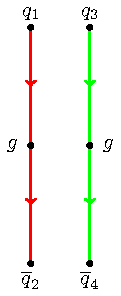
\includegraphics[width=\w\linewidth] {ColorDiagram_1_Individual}}; %b1
  \node (b2) at (2,0)  {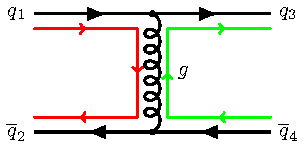
\includegraphics[width=\W\linewidth] {ColorDiagram_1_Diagram}}; %b1
  \draw[shorten >=0.8cm,shorten <=0.8cm,->, very thick] (b1)--(b2) node[midway,above=0.2] {Color flow to Feynman diagram};
\end{tikzpicture}
\end{document}